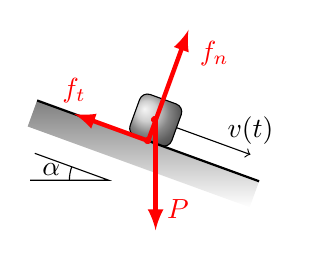
\begin{tikzpicture} [scale=1]%,font=\footnotesize]
	% bloc
	\draw[ball color=lightgray,rounded corners=3pt,rotate=-20] (-8pt,0) rectangle (8pt,16pt);
	% support
	\shade[bottom color=white,top color=gray,rotate=-20](-1.5,0)rectangle(1.5,-10pt);
	\draw[shift={(-.5,-.5)}](-1,0)--++(1,0)--++(160:1);
	\draw[shift={(-.5,-.5)}](-.5,0)arc(180:160:.5);
	\draw[shift={(-.5,-.5)}](170:.5)node[left, yshift=0.5mm]{$\alpha$};
	
	\draw[thick,rotate=-20] (-1.5,0)--++(3,0);	
	% vitesse
	\draw[->,rotate=-20](8pt,8pt)--++(1,0)node[above]{$\vv{v}(t)$};
	% forces
	\draw[-latex, ultra thick,red,rotate=-20](0,0)node{\tiny•}--++(-1,0)node[above]{$\vv{f_\text{t}}$};
	\draw[-latex, ultra thick,red,rotate=-20](0,0)--++(0,1.5)node[below right]{$\vv{f_\text{n}}$};
	\draw[-latex, ultra thick,red](2.7pt,7.5pt)node{\tiny•}--++(0,-1.4)node[above right]{$\vv{P}$};
\end{tikzpicture} 